\resizebox{0.65\textwidth}{!}{

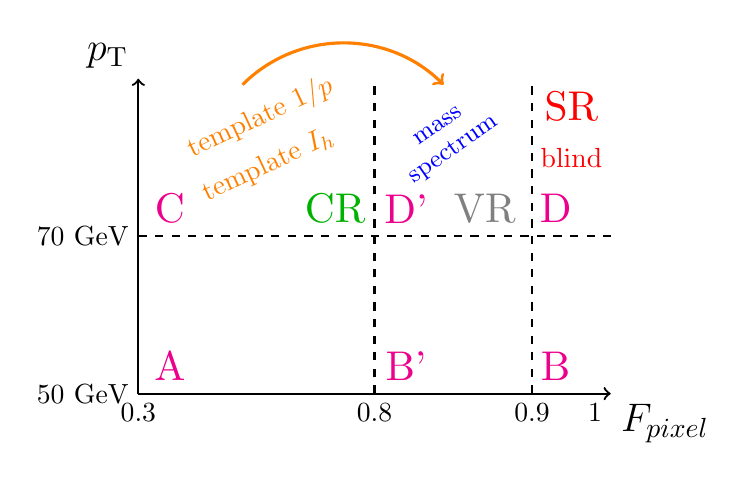
\begin{tikzpicture}

    % Axes
    \draw[->, thick] (0,0) -- (6,0) node[below right] {\Large$F_\text{pixel}$};
    \draw[->, thick] (0,0) -- (0,4) node[above left] {\Large $p_{\mathrm{T}}$};

    % Horizontal and vertical dashed lines
    \draw[dashed, thick] (3,0) -- (3,4); % x = 0.8
    \draw[dashed, thick] (5,0) -- (5,4); % x = 0.9
    \draw[dashed, thick] (0,2) -- (6,2); % y = 70 GeV

    % Region labels
    \node[green!70!black, scale=1.5] at (2.5,2.35) {CR};
    \node[gray, scale=1.5] at (4.4,2.35) {VR};
    \node[red, scale=1.5] at (5.5,3.65) {SR};

    \node[magenta, scale=1.5] at (0.4,2.35) {C};
    \node[magenta, scale=1.5] at (0.4,0.35) {A};
    \node[magenta, scale=1.5] at (3.4,2.35) {D'};
    \node[magenta, scale=1.5] at (5.3,2.35) {D};
    \node[magenta, scale=1.5] at (3.4,0.35) {B'};
    \node[magenta, scale=1.5] at (5.3,0.35) {B};
    
    
    % Text and arrows
    \node[rotate=25, orange] at (1.55,3.5) {template $1/p$};
    \node[rotate=25, orange] at (1.65,2.9) {template $I_h$};
    \node[rotate=35, blue] at (3.8,3.4) {\small mass};
    \node[rotate=35, blue] at (4,3.1) {\small spectrum};
    \node[rotate=0, red] at (5.5,3) {blind};
    
    \node (a) at (1.2,3.8) {};
    \node (b) at (4,3.8) {};
    \node (c) at (6.1,1.2) {};
    \node (d) at (5.8,3) {};
    \draw [->,orange,line width=0.4mm] (a) edge [bend left=45] (b);

    % Axis labels
    \node[below] at (5.8,0) {1};
    \node[below] at (5,0) {0.9};
    \node[below] at (3,0) {0.8};
    \node[below] at (0,0) {0.3};
    \node[left] at (0,2) {70 GeV};
    \node[left] at (0,0) {50 GeV};
    
\end{tikzpicture}

}